% !TeX spellcheck = de_CH
%%%%%%%%%%%%%%%%%%%%%%%%%%%%%%%%%%%%%%%%%%%%%%%%%%%%%%%%%%%%%%%%%
%  _____   ____  _____                                          %
% |_   _| /  __||  __ \    Institute of Computitional Physics   %
%   | |  |  /   | |__) |   Zuercher Hochschule Winterthur       %
%   | |  | (    |  ___/    (University of Applied Sciences)     %
%  _| |_ |  \__ | |        8401 Winterthur, Switzerland         %
% |_____| \____||_|                                             %
%%%%%%%%%%%%%%%%%%%%%%%%%%%%%%%%%%%%%%%%%%%%%%%%%%%%%%%%%%%%%%%%%
%
% Project     : BA Welti Keller
% Title       : 
% File        : anhang.tex Rev. 00
% Date        : 15.09.2014
% Author      : Tobias Welti
%
%%%%%%%%%%%%%%%%%%%%%%%%%%%%%%%%%%%%%%%%%%%%%%%%%%%%%%%%%%%%%%%%%


\pagenumbering{Roman}

\appendix
\chapter{Anhang}\label{chap.anhang}

\todo{Anhang}

\section{Offizielle Aufgabenstellung}\label{app.aufgabenstellung}
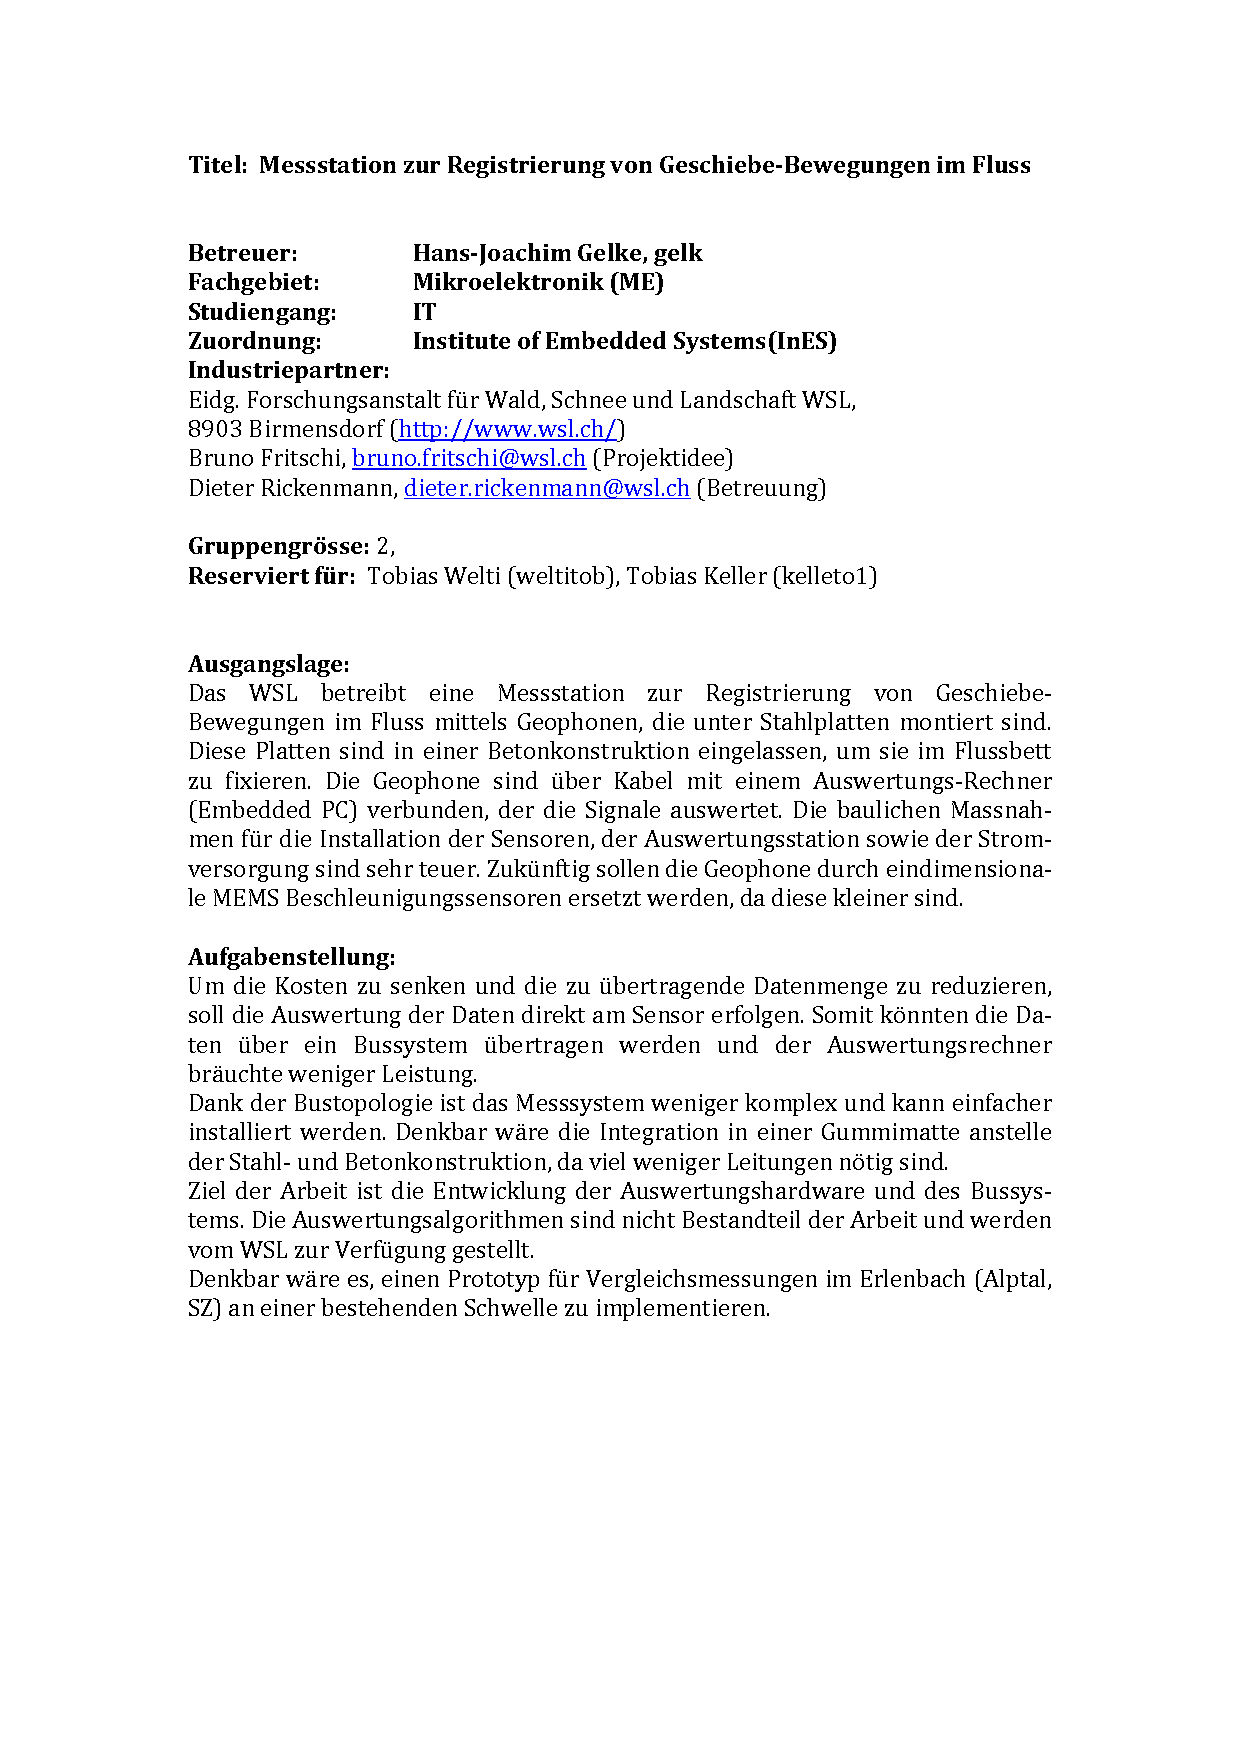
\includepdf{images/BA_welti_keller_hs14.pdf}


\section{Projektmanagement}\label{app.projektmanagement}

\subsection{Zeitplan}
\todo{Zeitplan}

\subsection{Besprechungsprotokolle}

\subsubsection{Projektskizzierung an der WSL, Birmensdorf}
Die erste Sitzung zum Projekt fand am 16. Juli 2014 an der \gls{wsl} in Birmensdorf statt. Anwesende waren Bruno Fritschi (Projektidee), Carlos Wyss (Doktorand), Alexandre Badoux (Gruppenleiter) sowie Tobias Keller und Tobias Welti.

Die Projektidee wurde von Bruno Fritschi noch einmal erklärt. Carlos Wyss zeigte einige Beispiele von bestehenden Messresultaten und erläuterte den Algorithmus der \gls{ereignisdet}, die mittels Hilbert-Transformation gelöst wird. Die Datenreduktion erfolgt durch Berechnung eines Histogramms der Peakintensitäten über eine Minute und die Speicherung der Dauer, Intensität und Anzahl \glspl{peak} jedes \gls{ereignis}ses. Als minimale Anforderung an die Messdaten wurde vereinbart, dass die \gls{fs} mindestens 10~kHz beträgt und mindestens die gleichen Werte gespeichert werden wie bisher.

Als Wunsch wurde von Carlos Wyss geäussert, die Originaldaten von Anfang bis Ende der \gls{ereignis} speichern zu können.


\subsubsection{Zwischenbesprechung an der ZHAW, Winterthur}
Eine Zwischenbesprechung am 28. Oktober 2014 an der ZHAW Winterthur verlief sehr zufriedenstellend. Anwesend waren Prof. Hans Gelke (Betreuer), Bruno Fritschi sowie Tobias Keller und Tobias Welti.

\paragraph{Projektstand} An der Zwischenbesprechung konnte bereits der Testaufbau mit einer \gls{sensoreinh} vorgeführt werden. Die Signale wurden auf einem Oszilloskop visualisiert und entsprachen den Erwartungen von Bruno Fritschi. Die Dimensionen der Geräte waren jedoch wesentlich grösser als erwartet. 

\paragraph{Beschlüsse} In der Diskussion wurde entschieden, die bereits im Aufbau befindlichen Gehäuse trotzdem fertig zu bauen. Das Projekt war zu diesem Zeitpunkt auf einem guten Weg, weshalb keine Massnahmen oder Änderungen an den Zielen beschlossen wurden.

\subsubsection{Zwischenbesprechung an der VAW, ETH Hönggerberg}
Am 12. November 2014 fand eine zweite Projektsitzung statt, diesmal an der \gls{vaw} an der ETH Hönggerberg. Anwesend waren Prof. Hans Gelke, Prof. Dieter Rickenmann (WSL), Bruno Fritschi, Carlos Wyss sowie Tobias Keller und Tobias Welti.

\paragraph{Projektstand} Die Methode der Ereigniserkennung mittels einer State Machine mit konfigurierbaren Parametern wurde vorgestellt und von den Anwesenden gelobt. Die verschiedenen Detail-Level wurden intensiv diskutiert und Vor- und Nachteile aufgeführt. 

\paragraph{Beschlüsse} Es wurde beschlossen, das Projekt mit allen vorgeschlagenen Detail-Levels weiterzuführen, da für jeden Modus ein plausibles Szenario gefunden wurde. Da das Projekt mit der \gls{ereignisdet} und Teilen des CAN-Protokolls gut im Zeitplan lag, wurden keine Änderungen der Ziele definiert. Die geplanten Tests an der \gls{vaw} wurden aber auf einen Zeitpunkt nach dem Abschluss der Bachelorarbeit verschoben.

Für die Tests in der Versuchsrinne ist vorgesehen, die Sensoren ausserhalb der Gehäuse der \glspl{sensoreinh} anzuschliessen und unter die bestehende Stahlplatte zu montieren. Dann können Vergleichsmessungen mit Geophonen und \gls{mems}-Beschleunigungssensoren durchgeführt werden.

Als Folgeprojekt oder möglicher Entwicklungsauftrag an die ZHAW wurde die Miniaturisierung  der \gls{sensoreinh} und deren Entwicklung zur Produktreife ins Auge gefasst.

Im Anschluss an die Sitzung wurde die \gls{vaw} besichtigt. Hier konnten sich die Entwickler zum ersten Mal ein (eindrückliches!) Bild der bestehenden Messinstallationen mit Geophonen machen.

\section{Schaltpläne}\label{app.pcb}
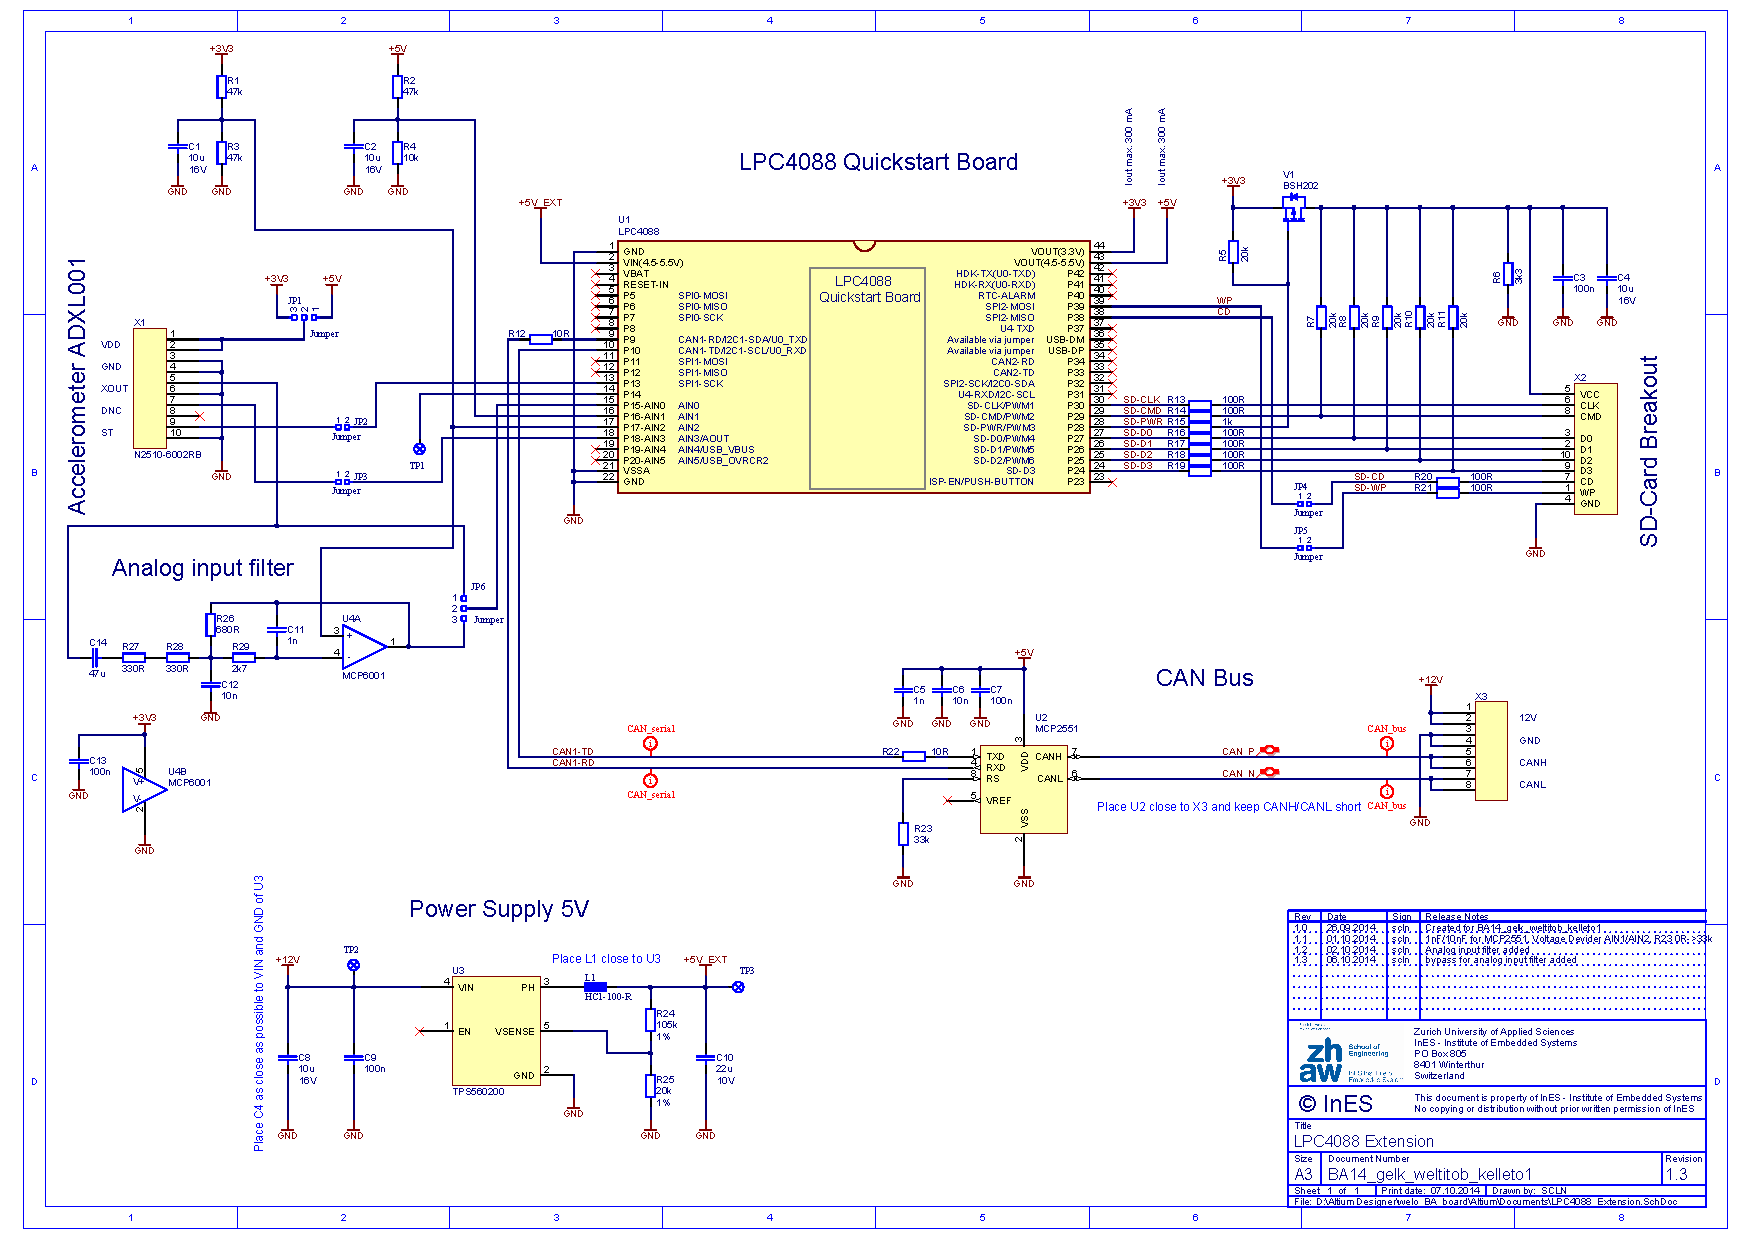
\includepdf[angle=90]{images/pcb/Schematic.pdf}
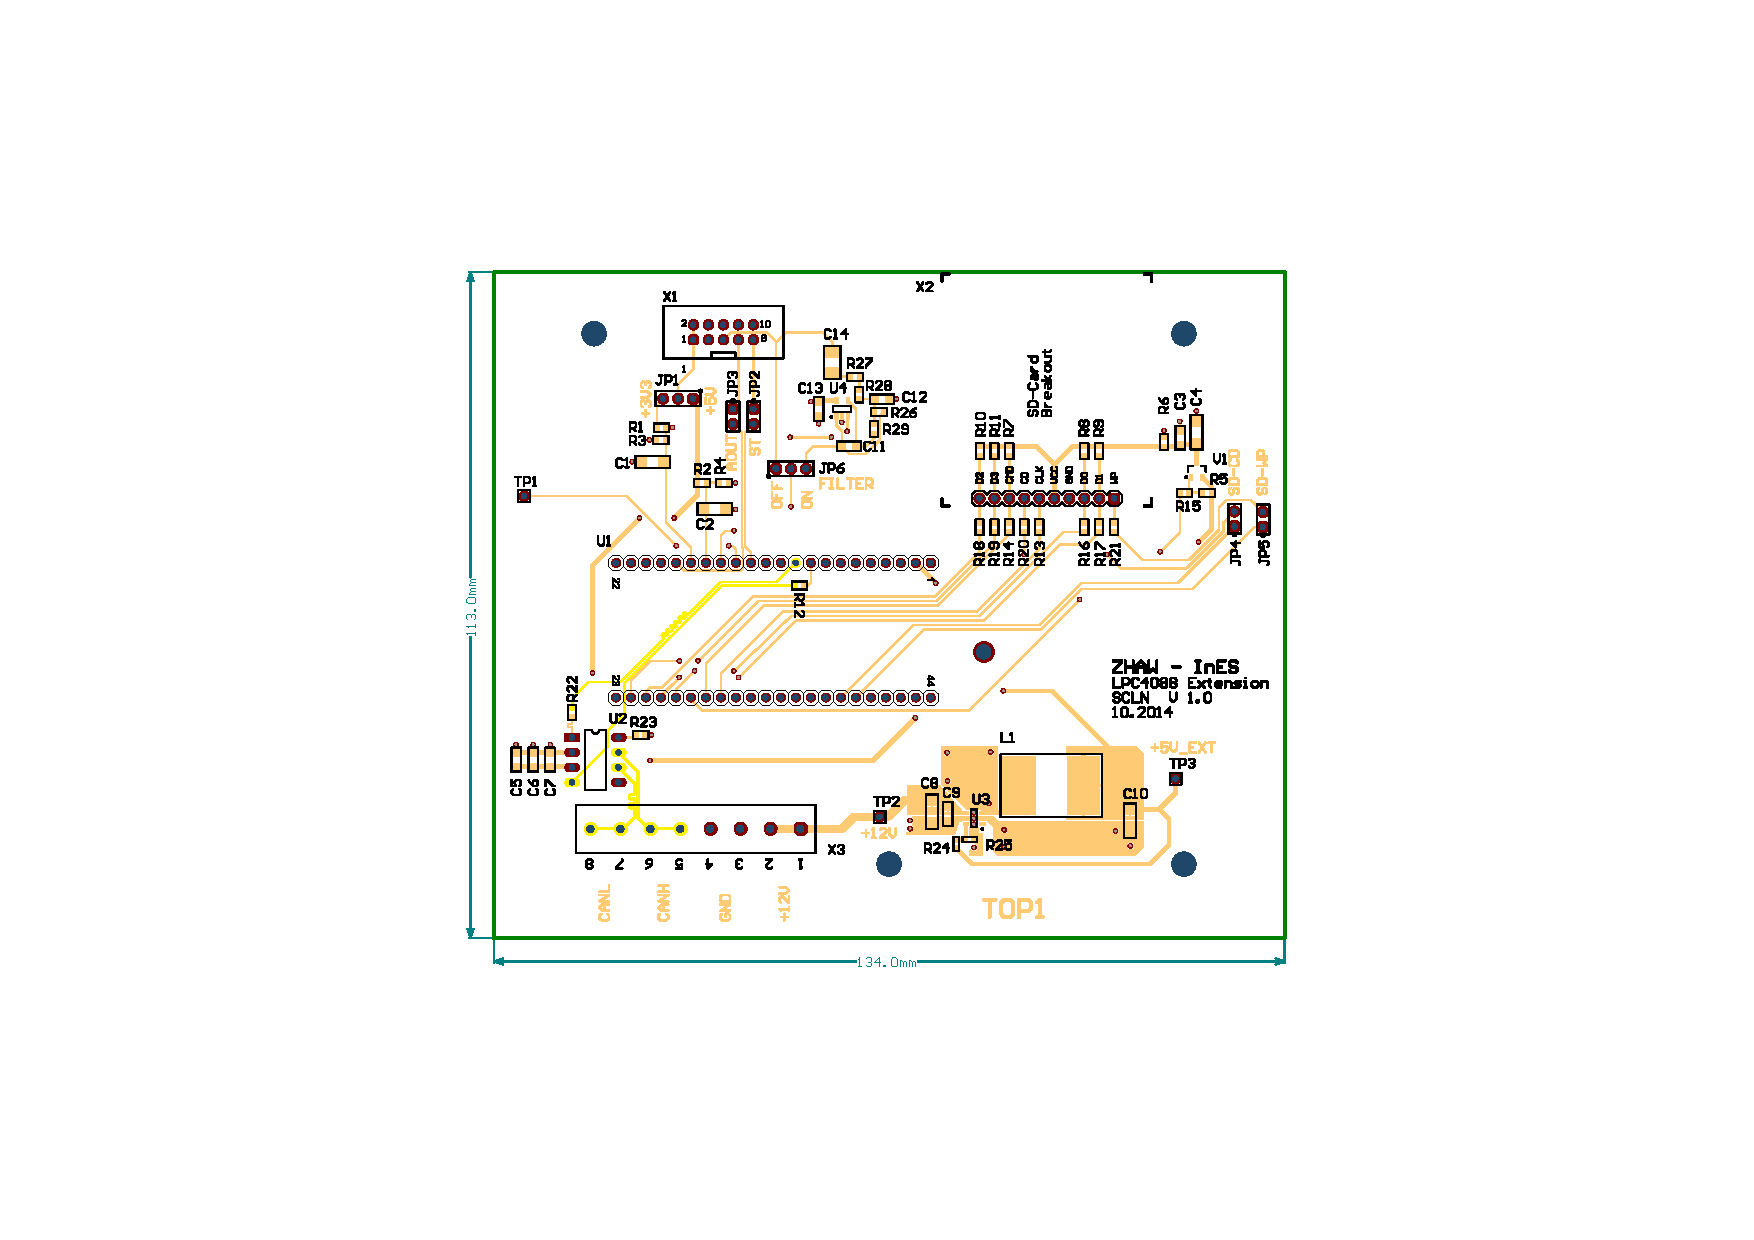
\includepdf[pages={1,2},angle=90]{images/pcb/PCB_Layout.pdf}


\section{Datenblätter}\label{app.datasheets}
Um die Dokumentation übersichtlich zu halten, wird der Grossteil der Datenblätter nicht mit der Dokumentation ausgedruckt, sondern auf der beiliegenden \gls{cd} mitgeliefert.


\subsection{NXP LPC4088 32-bit ARM Cortex-M4 microcontroller}

\includepdf[pages={7}]{images/datasheets/LPC408X_7X.pdf}\label{ds.lpc4088}


\subsection{Embedded Artists NXP LPC4088 QuickStart Board}

\begin{figure}[H]
	\centering		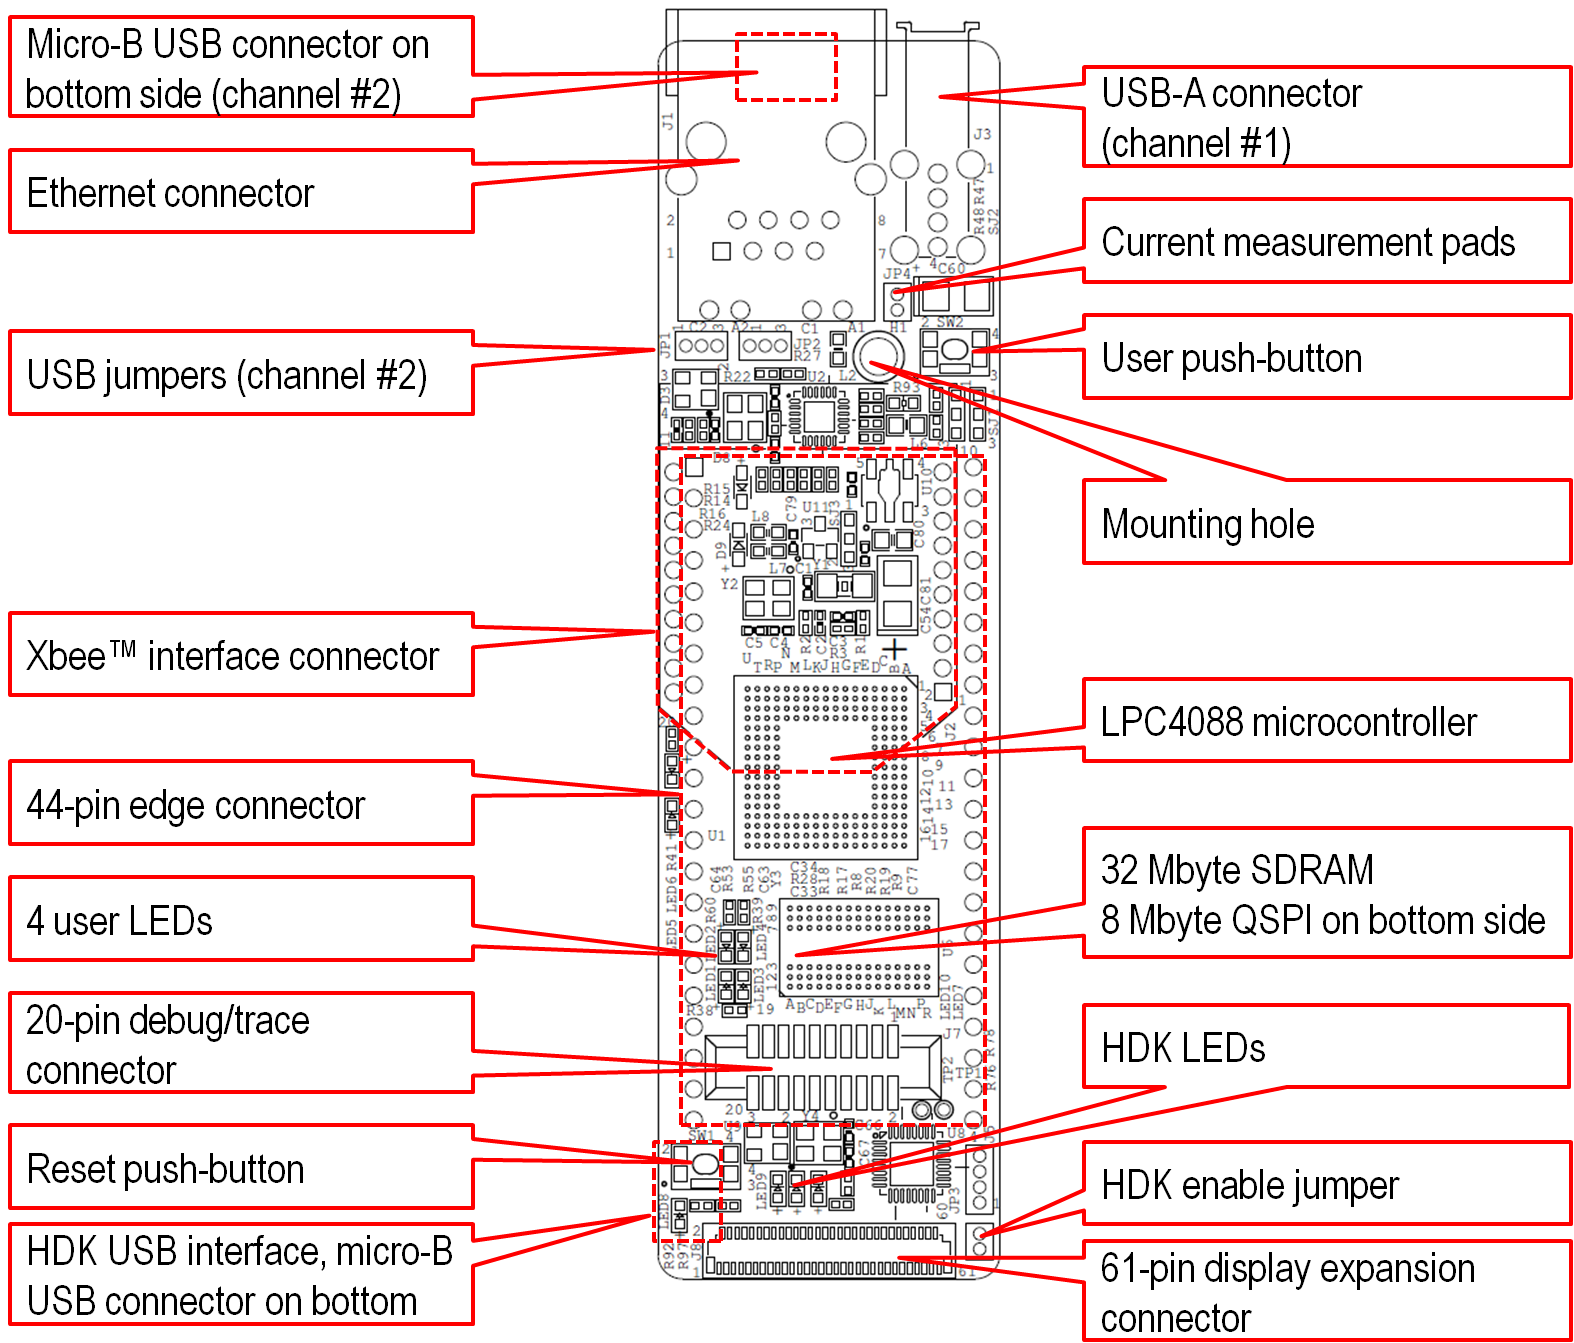
\includegraphics[width=0.7\textwidth]{images/datasheets/lpc4088_qsb_key_components_reva.png}
	\caption{Hauptkomponenten des NXP LPC4088 QuickStart Boards von Embedded Artists.}
	\label{fig.NXP_LPC4088_QSB_comps}
\end{figure}

\begin{figure}[H]
	\centering		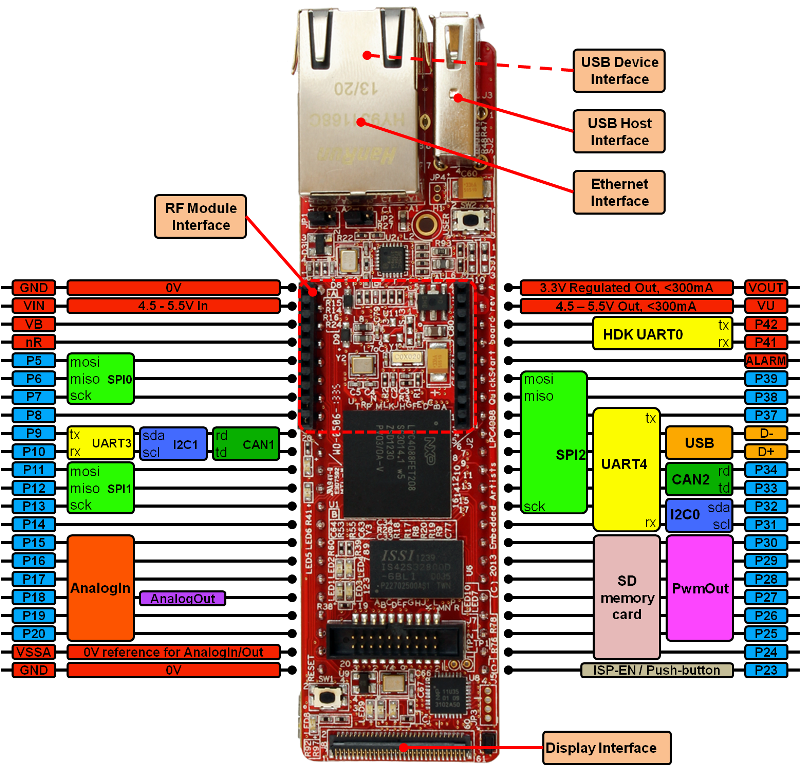
\includegraphics[width=0.7\textwidth]{images/datasheets/LPC4088_QSB_pinning_revA_800x769.png}
	\caption{Pins des NXP LPC4088 QuickStart Boards von Embedded Artists.}
	\label{fig.NXP_LPC4088_QSB_pinout}
\end{figure}

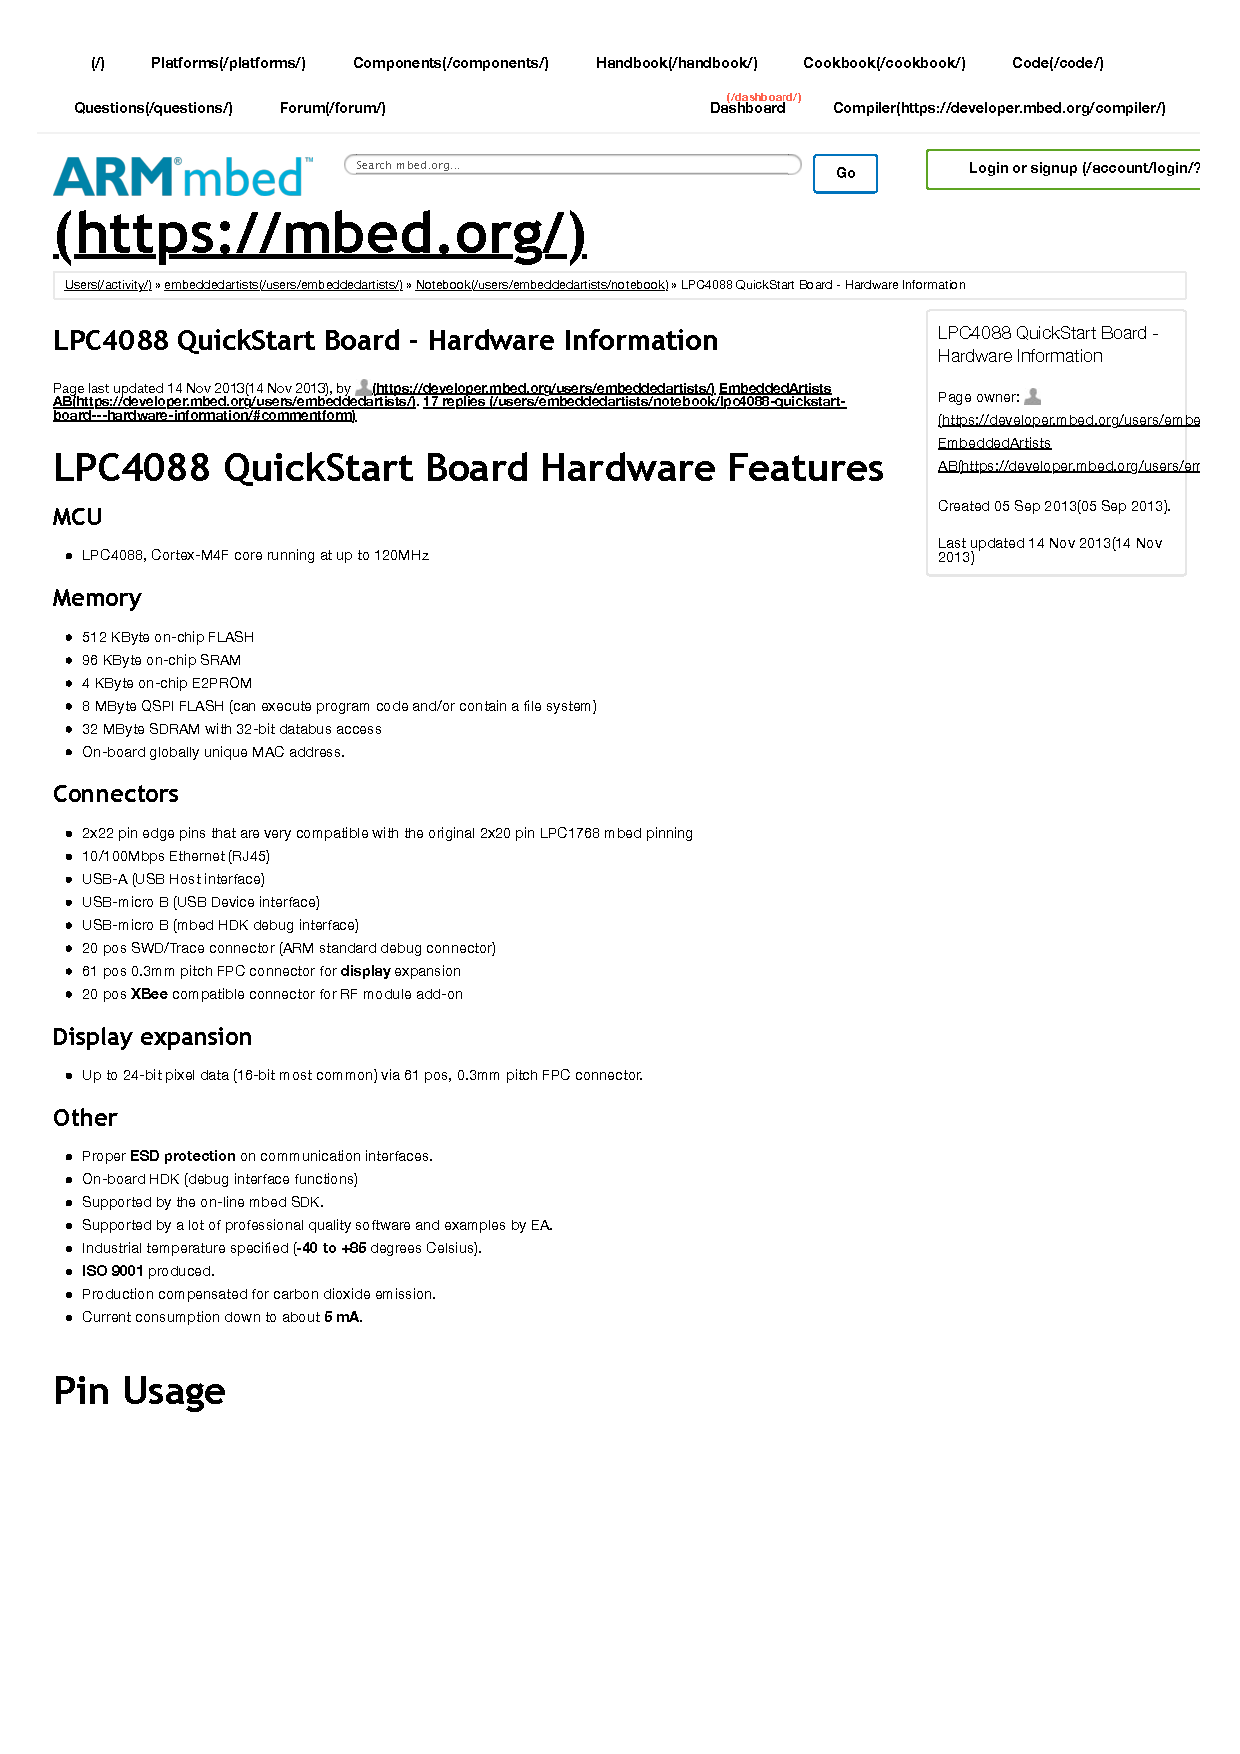
\includepdf{images/datasheets/LPC4088qsb.pdf}

\subsection{Analog Devices ADXL001 Beschleunigungssensor}
\includepdf[pages={3}]{images/datasheets/ADXL001.pdf}


\section{Fotos}\label{sec.foto.testaufbau}
Die Fotos befinden sich auf der beiliegenden CD und können auch aus dem Git-Repository unter \url{https://github.com/tokeller/WeKeBA} heruntergeladen werden.

\section{Source Code, Daten und Multimedia}\label{app.cd}
Da der Source Code sehr umfangreich ist, wird darauf verzichtet, ihn ausgedruckt zur Verfügung zu stellen. Er befindet sich auf der beiliegenden \gls{cd}.

\todo{Inhaltsverzeichnis der CD erstellen\\
CD mit dem vollständigen Bericht als pdf-File inklusive Film- und Fotomaterial}
